\section{Problem Statement} \label{sec:problem-statement}

\tool phrases alignment as a probabilistic inference task that we introduce and motivate in this section. The inference task is based on a generative model that specifies how reads are generated. A mathematically precise formulation of this generative model ensures that \tool solves the correct alignment task.

\para{Notation}
\cref{tab:notation} provides a summary of notation used in this work.
The first two parts of \cref{tab:notation} provide a quick reference for the notation introduced in this section.
For now, we only note that we distinguish sets of instances (\eg $\genomes$), random variables inducing a distribution over these sets (\eg $G$), and instances of random variables (\eg $g$).

The last part of \cref{tab:notation} summarizes notation we use without further comments.
The only non-standard notation is $\genome\llbracket i \rrbracket$ (and $\genome\llbracket i \shortcolon j \rrbracket$), which we use to indicates the positions at which a given read could align.
Formally, we can interpret $\genome\llbracket i \rrbracket$ as the tuple $(\genome,i)$.

% We use standard, but explicit notation to indicate the probability of events. For example, to indicate the probability of alignment $a$, conditioned on observing the read $s$, we write

% Here, the subscripts $A,S^\gread$ explicitly indicate that the probability is over the joint distribution of $A$ and $S^\gread$.
% We note that this notation allows $A$ and $S^\gread$ to be correlated.

% The symbol $\graph$ stands for graph representing a random variable over genome segments. 

\begin{table}
	\centering
	\small
	\begin{tabular}{ c c c c }
		& Set & Random Variable & Instance \\
		Genome & $\genomes$, $\genomes^\gcore$, $\genomes^\gmut$ & $\genomeRV$, $\genomeRV^\gcore$, $\genomeRV^\gmut$ & $\genome$, $\genome^\gcore$, $\genome^\gmut$ \\
		Alignment & $\alignments$ & $\alignmentRV$ & $\alignment$, $\alignment^\star$ \\
		Genome Segment & $\segments$, $\segments^\gread$ & $\segmentRV$, $\segmentRV^\gread$ & $\segment$, $\segment^\gread$ \\
		Start of segment & $\{0,\dots,\abs{\genome}-1 \}$ & $\startInGenomeRV$, $\startInGenomeRV^\gmut$ & $\startInGenome$, $\startInGenome^\gmut$
	\end{tabular} \\
	%\fullline \\
	\begin{tabular}{ l c }
		\\[-1em] \hline \\[-1em]
		% Meaning of superscript & Usages \\
		Superscript indicating core genome & $^\gcore$ \\ % , as in $\genomes^\gcore$, $\genomeRV^\gcore$, $\genome^\gcore$
		Superscript indicating mutated genome & $^\gmut$ \\ % , as in $\genomes^\gmut$, $\genomeRV^\gmut$, $\genome^\gmut$ / $\startInGenomeRV^\gmut$, $\startInGenome^\gmut$
		Superscript indicating read of genome segments & $^\gread$ \\ % , as in $\segments^\gread$, $\segmentRV^\gread$, $\segment^\gread$
		\\[-1em] \hline \\[-1em]
		Letter at \nth{i} position of genome $\genome$ ($0$-based indexing) & $\genome[i]$ \\
		Position $i$ in genome $\genome$ & $\genome \llbracket i \rrbracket$ \\
		Letters/Positions $i$ (inclusive) to $j$ (exclusive) of genome $\genome$ & $\genome[i \shortcolon j]$, $\genome \llbracket i \shortcolon j \rrbracket$ \\
		Length of genome or segment & $\abs{\genome}$, $\abs{\segment}$ \\
		Set of paths of length $L$ in graph $\graph$ & $\paths{L}{\graph}$
	\end{tabular}
	\caption{Summary of notation.}
	\label{tab:notation}
\end{table}

\para{Inspiration: Complete Genomes Model}
Our generative model is inspired by a model of biological reality, depicted in the first column of \cref{fig:models}.

It starts from a random variable $\genomeRV$ over the set $\genomes = \{\genome_i\}_{i \in \mathcal{I}}$ of haploid genomes occurring in the population under consideration.
The genomes in $\genomes$ exhibit both small-scale and large-scale variations appearing in the population.
Small-scale variations include de-novo mutations and other rare mutations, while large-scale variations capture common mutations in the population that typically span multiple base pairs.
The distribution of the random variable $\genomeRV$ captures the probability of each genome $\genome$.
We note that this distribution is typically not uniform, as some variations are more common than others.
As a consequence, ignoring the distribution of $\genomeRV$ (as done, \eg by the Smith-Waterman algorithm) will necessarily lead to loss of information.

The model first samples a genome $\genome$ from $\genomeRV$.
Then, it sequences $\genome$, resulting in a read $\segment^\gread$ of a predetermined length $L$.
Sequencing consists of (i)~randomly chopping the genome into smaller segments, (ii)~discarding segments shorter than $L$ and selecting one remaining segment $\segment$ of length at least $L$ to read, and (iii) reading the first $L$ letters in $\segment$, resulting in $\segment^\gread$.
In general, $\segment \neq \segment^\gread$ even if the length of $\segment$ is $L$, as reading is noisy and may introduce \emph{read errors}.

We assume the model does not only report the read $\segment^\gread$, but also the probability of reading each letter correctly.
Typically, this probability is represented as a phred quality score \cite{ewing_base-calling_1998}:
$$Q_i := -10 \cdot \log_{10}\Pr{\text{error reading \nth{i} letter}},$$
However, we work with phred probabilities instead, denoted by
$$
\pphred{i} := \Pr{\text{correctly reading \nth{i} letter}}.
$$


\subsection{Our Model: Core Genomes Model} \label{sec:generative-model}
%In this section, we describe the generative model underlying our inference task.
Instantiating the Complete Genomes Model in practice is impossible; we typically cannot even enumerate all genomes in $\genomes$.
Instead, we introduce the Core Genomes Model, which starts from a random variable $\genomeRV^\gcore$ over a set $\genomes^\gcore$ of \emph{core genomes}.
In contrast to $\genomes$, the core genomes in $\genomes^\gcore$ only capture the large-scale variations appearing in the population.

\para{Mutations}
Our model introduces small-scale variations by first sampling a core genome $\genome^\gcore$ from $\genomeRV^\gcore$ and then mutating it.
To mutate $\genome^\gcore$, our model copies it letter by letter, generating a mutated genome $\genome^\gmut$.
When the model is about to copy the \nth{i} letter of $\genome^\gcore$, it probabilistically decides to (i)~insert a new letter (insertion), (ii)~skip this letter (deletion), (iii)~copy the letter incorrectly (edit), or (iv)~copy the letter correctly (copy).

\begin{figure}
	\lstinputlisting[language=MyPython,caption={Code for mutating a core genome.},label={lst:mutate-minified}]{code/mutate_minified.py}
\end{figure}

\cref{lst:mutate-minified} shows an algorithmic description of this mutation process.
It iterates over the positions \texttt{i} in $\genomes^\gcore$ and and in every step determines all possible actions (\crefrange{line:mutate-actions-def}{line:mutate-actions-select}).
Each action consists of a probability for that action, an action type (insertion, deletion, edit, copy), and the letter produced by this action ($\epsilon$ indicates no letter, for deletions).
Unless the action is a deletion, \cref{lst:mutate-minified} appends the new letter to the mutated genome (\crefrange{line:mutate-del-check}{line:mutate-no-del}).
Then, unless the action is an insertion, \cref{lst:mutate-minified} advances the read pointer (\crefrange{line:mutate-ins-check}{line:mutate-no-ins}).

For simplicity of presentation, \cref{lst:mutate-minified} assumes that each action type occurs with a constant probability at every position. 
In addition, it assumes that the new letter for insertions and edits is selected uniformly at random from all letters, \ie each letter has a probability of $\pins/4$ to be inserted.
Likewise, the process selects the new letter for edits uniformly at random from all letters different from the current one, \eg copying letter $A$ yields (edited) letter $C$, $G$, or $T$ with a probability of $\ped/3$, respectively.
It is straightforward to extend \cref{lst:mutate-minified} to allow for position-dependent action probabilities, and for a selection of new letters according to a different distribution.

In \cref{line:mutate-return}, \cref{lst:mutate-minified} does not only return the mutated genome $\genome^\gmut$, but also its mutation history \texttt{mutations}, constructed in \cref{line:mutate-history}.
For every step in the mutation process, the history records (i)~the current position of the read pointer consisting of $\genome^\gcore$ and \texttt{i}, (ii) the action type (\texttt{action}), and (iii)~the generated letter (\texttt{letter}).

\para{Sequencing}
After determining $\genome^\gmut$, our model sequences it according to the following steps (these steps formalize the sequencing process described in the Complete Genomes Model).

First, it selects a starting point $\startInGenome$ in $\genome^\gmut$ by sampling from a random variable $\startInGenomeRV$ describing the distribution over all possible starting points.
To avoid reads of length less than $L$, $\startInGenomeRV$ must never select one of the last $L-1$ positions of $\genome$.

Second, our model determines the segment $\segment := \genome[\startInGenome \shortcolon \startInGenome+L]$.
We note that unlike the Complete Genomes Model, our model does not produce longer segments than $L$ at this stage.
Since the read only depends on the first $L$ letters of $\segment$, this simplification does not affect the behavior of our model.

\begin{figure}
	\lstinputlisting[language=MyPython,caption={Code for reading a sequence.},label={lst:read-minified}]{code/read_minified.py}
\end{figure}

Finally, our model reads $\segment$ letter by letter in order to produce $\segment^\gread$.
We provide an algorithmic description of the read process in \cref{lst:read-minified}.
For every letter, the model may (i)~read it correctly with probability \texttt{1-p\_error}, or (ii)~read it incorrectly with probability \texttt{p\_error}.
Analogously to the mutation process, for simplicity of presentation, \cref{lst:read-minified} assumes constant error probabilities and a selects erroneous letters uniformly at random.
Likewise, \cref{line:read-return} does not only return the sequenced read $\segment^\gread$, but also its read error history \texttt{errors}, constructed in \cref{line:read-history}.
For every read letter, the history records (i)~the current position of the read pointer, (ii)~the action type, and (iii)~the generated letter.

% We assume that if $\genomes^\gcore$ and the mutation process are selected appropriately, capturing large-scale and small-scale variations respectively, then $\genome^\gmut$ follows the same distribution as $\genome$ sampled from $\genomes$.
% Under this assumption, the Core Genomes Model is equivalent to the Complete Genomes Model.

\begin{figure}
	\centering
	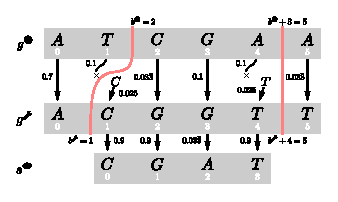
\includegraphics[width=0.99\linewidth]{figures/edit-example}
	\caption{Generation of a read $\segment^\gread=CGAT$ from core genome $\genome^\gcore=ATCGAA$ by editing and sequencing. Arrows indicate copied letters ($\pcopy=0.7$) or edited (dashed arrow; $\ped=0.1$), inserted (arrow starting from a new letter; $\pins=0.1$), or deleted (arrow to x; $\pdel=0.1$). During sequencing, we assume a phred probability of $\pphred{i} = 0.9$ at every position $i$.}
	\label{fig:alignment-full}
\end{figure}

\para{Example}
\cref{fig:alignment-full} shows the full process of generating $\segment^\gread$ on a concrete example.
The model first selects a core genome $\genome^\gcore=ATCGAA$.
Then, it copies $\genome^\gcore$ letter by letter, generating the mutated genome $\genome^\gmut=ACGGTT$.
The numbers in \cref{fig:alignment-full} indicate the probabilities of each action.
Overall, the probability of generating $\genome^\gmut$ from $\genome^\gcore$, according to the depicted actions, is $0.7 \cdot 0.1 \cdot 0.025 \cdot 0.03\bar{3} \cdot 0.1 \cdot 0.1 \cdot 0.025 \cdot 0.03\bar{3} \approx 5 \cdot 10^{-10}$.
We note there are other actions that can also generate $\genome^\gmut$ from $\genome^\gcore$, \eg instead of editing $C$ to $G$, the model could delete $C$ and insert $G$.

After generating $\genome^\gmut$, the model selects a starting position $\startInGenome^\gmut=1$ and copies the $L=4$ letters $\genome^\gmut[1 \shortcolon 5]$ to generate $\segment^\gread$.
The probability of generating $\segment^\gread$ from $\genome^\gmut$ is $0.9 \cdot 0.9 \cdot 0.03\bar{3} \cdot 0.9 \approx 2.4 \cdot 10^{-2}$.

\subsection{Alignment as an Inference Task} \label{sec:alignment}
In this section, we define the alignment task as an inference task in the generative model introduced in \cref{sec:generative-model}.
Our generative model induces a genome alignment task: Given a read $\segment^\gread$, determine its generation history consisting of the mutation history and the read error history leading to $\segment^\gread$.

Generally, given the mutation history and the read $\segment^\gread$, the read error history can be reconstructed.
In addition, the mutation history describes the generation of the full $\genome^\gmut$, even though $\segment^\gread$ may only provide information about the generation of $\genome^\gmut[\startInGenome \shortcolon \startInGenome + L]$. 
Therefore, we define the alignment $\alignment$ of $\segment^\gread$ to be its mutation history, restricted to positions $\startInGenome^\gmut$ to $\startInGenome^\gmut + L$.
%In terms of the algorithmic description in \cref{lst:mutate-full}, $\alignment = \texttt{history}[\startInGenome^\gmut:\startInGenome^\gmut+L]$.

\para{Example}
In \cref{fig:alignment-full}, alignment only considers the mutations occurring
between the red lines. Concretely, \cref{fig:alignment-full} induces alignment
$\alignment$, given by 
\begin{align*}
&(\genome^\gcore\llbracket 2 \rrbracket,\text{ins},C),(\genome^\gcore\llbracket 2 \rrbracket,\text{edit},G), (\genome^\gcore\llbracket 3 \rrbracket,\text{copy},G),\\
&(\genome^\gcore\llbracket 4 \rrbracket,\text{del},\epsilon),(\genome^\gcore\llbracket 5 \rrbracket,\text{ins},T).
\end{align*}

We note that $\alignment$ does not include the deletion of $T$, as it occurred before generating the first letter from $\segment^\gread$.
Likewise, it does not include deletions that occur after generating the last letter from $\segment^\gread$.

\para{\acs{map} Alignment}

Given only $\segment^\gread$ from \cref{fig:alignment-full}, there are more likely alignments than $\alignment$.
For example, instead of deleting $\alignment$ from $\genome^\gcore$ and inserting $T$ into $\genome^\gmut$, editing $A$ to $T$ would be a more likely explanation.
Generally, we can not hope to always identify the true alignment of a read, but we can determine the most likely alignment $\alignment^\star$, given the read $\segment^\gread$. This corresponds to \acf{map} estimation, and can be written as:
\begin{align} \label{eq:MAP-alignment}
	\alignment^\star = \argmax_{\alignment} \Pr{\alignmentRV=\alignment \mid \segmentRV^\gread = \segment^\gread}
\end{align}

In \cref{eq:MAP-alignment}, we are using random variables $\alignmentRV$ and $\segmentRV^\gread$ which are correlated: $\alignmentRV$ is the alignment of $\segmentRV^\gread$.

% \begin{figure}	
% \begin{tikzpicture}
% 	node distance=2.5cm, % Minimum distance between two nodes. Change if necessary.
% 	every state/.style={ % Sets the properties for each state
% 		semithick,
% 		fill=gray!10},
% 	initial text={}, % No label on start arrow
% 	double distance=2pt, % Adjust appearance of accept states
% 	every edge/.style={ % Sets the properties for each transition
% 		draw,
% 		->,>=stealth’, % Makes edges directed with bold arrowheads
% 		auto,
% 	semithick}

% 	\node[state, initial] (q1) {$q_1$};
% 	\node[state, right of=q1] (q2) {$q_2$};
% 	\node[state, right of=q2] (q3) {$q_3$};
% 	\node[state, right of=q3] (q4) {$q_4$};
% 	\node[state, accepting, right of=q4] (qN) {};

% 	\draw (q1) edge[loop above] node {\tt A,C,G,T} (q1);
% 	\draw (q1) edge[] node {\tt G} (q2);
% 	\draw (q1) edge[bend right=60] node {\tt A,C,G,T,$\epsilon$} (q2);

% 	\draw (q2) edge[loop above] node {\tt A,C,G,T} (q2);
% 	\draw (q2) edge[] node {\tt A} (q3);
% 	\draw (q2) edge[bend right=60] node {\tt A,C,G,T,$\epsilon$} (q3);

% 	\draw (q3) edge[loop above] node {\tt A,C,G,T} (q3);
% 	\draw (q3) edge[] node {\tt T} (q4);
% 	\draw (q3) edge[bend right=60] node {\tt A,C,G,T,$\epsilon$} (q4);

% 	\draw (q4) edge[loop above] node {\tt A,C,G,T} (q4);
% 	\draw (q4) edge[] node {\tt $\epsilon$} (qN);
% \end{tikzpicture}
% \end{figure}

% \para{MAP vs MLE} \todo{this paragraph does not fit here. I don't think it is relevant, can probably be deleted}
% In the context of MAP and MLE optimization during inference, the observed data is the query read and the mapping parameter is the resulting alignment.
% In case of a uniform distribution of the genomes in the core model, MAP mapping is equivalent to MLE mapping.
% Not weighting the starting positions in the graph models is indirectly stating some (possibly not uniform) prior distribution on the genomes and their positions.
% In order to translate a known core genomes prior of the genomes to the graph model, the edge weights have to be chosen or learned appropriately.


% \begin{itemize}
% 	\item desirable properties
% 	\item $3$ sources of uncertainty
% \end{itemize}
